% CREATED BY DAVID FRISK, 2015
\chapter{Evaluation and Results}
In this chapter, the efficiency of the mechanisms that were studied above will be analysed, on whether they can achieve targeted data extraction. The experiments that were carried out, as well as the results that will be presented below are divided in three units, depending on the kind of data we want to extract:\\
\begin{itemize}

	\item Argument Extraction (\ref{41_ref})
	\item Suggestion Extraction (\ref{42_ref})


\end{itemize}
\section{Argument Extraction}\label{41_ref}
In this subsection the results of the methods that were introduced in the previous chapters on the writer's argument extraction will be presented. In this subsection especially, we are going to try to present some indicators for the Argument Markers that we set. These indicators show the ``ability'' of each variable to ``find'' an Argument (\ref{411_ref}). Also, we are going to see the efficiency of each Algorithm that we tried in this procedure (\ref{412_ref}). Finally, we are going to present some diagrams that show the efficiency of the Train Set that we have created on the writer's Argument Extraction from the texts (\ref{413_ref}).

\subsection{Argument Markers}\label{411_ref}
As we saw above, the corpus that was studied had a total of 1015 sentences, which make up approximately two hundred users' texts (user commentaries). Initially, we need to stress that in the corpus, the number of sentences that were characterised as Argumentative is relatively bigger than the number of sentences that were not characterised as Argumentative. This property is shown in the following diagram.
\begin{figure}[H]
\centering
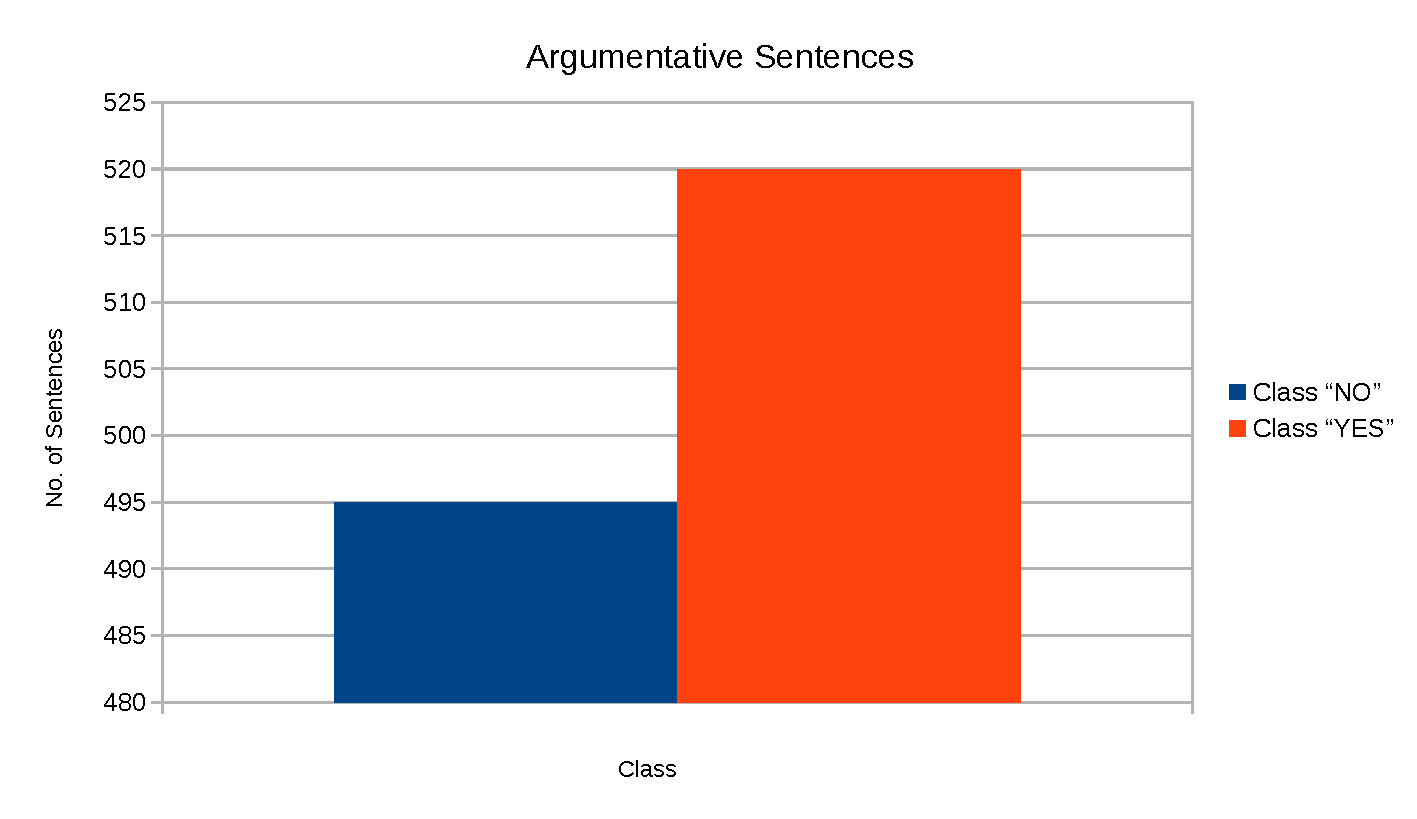
\includegraphics[width=0.9\linewidth]{figure/arguments/A_argumentative1.pdf}
\caption{Argumentative Sentences in Train Set.}
\end{figure}

In the rest of this unit (\ref{421_ref}), class ``yes'', i.e. the sentences that are ``Argumentative'' will be symbolised with red and respectively, the sentences belonging to class ``no'' will be symbolised with blue.\\
\\
In the next diagrams we can see  for each one of the Argument Markers that we have set, the ability of each variable to define an Argument. The axis X shows the frequency of each variable in each sentence. What we note in most diagrams, is that as frequency increases, class ``yes'' surpasses class ``no''.

\begin{figure}[H]
\centering
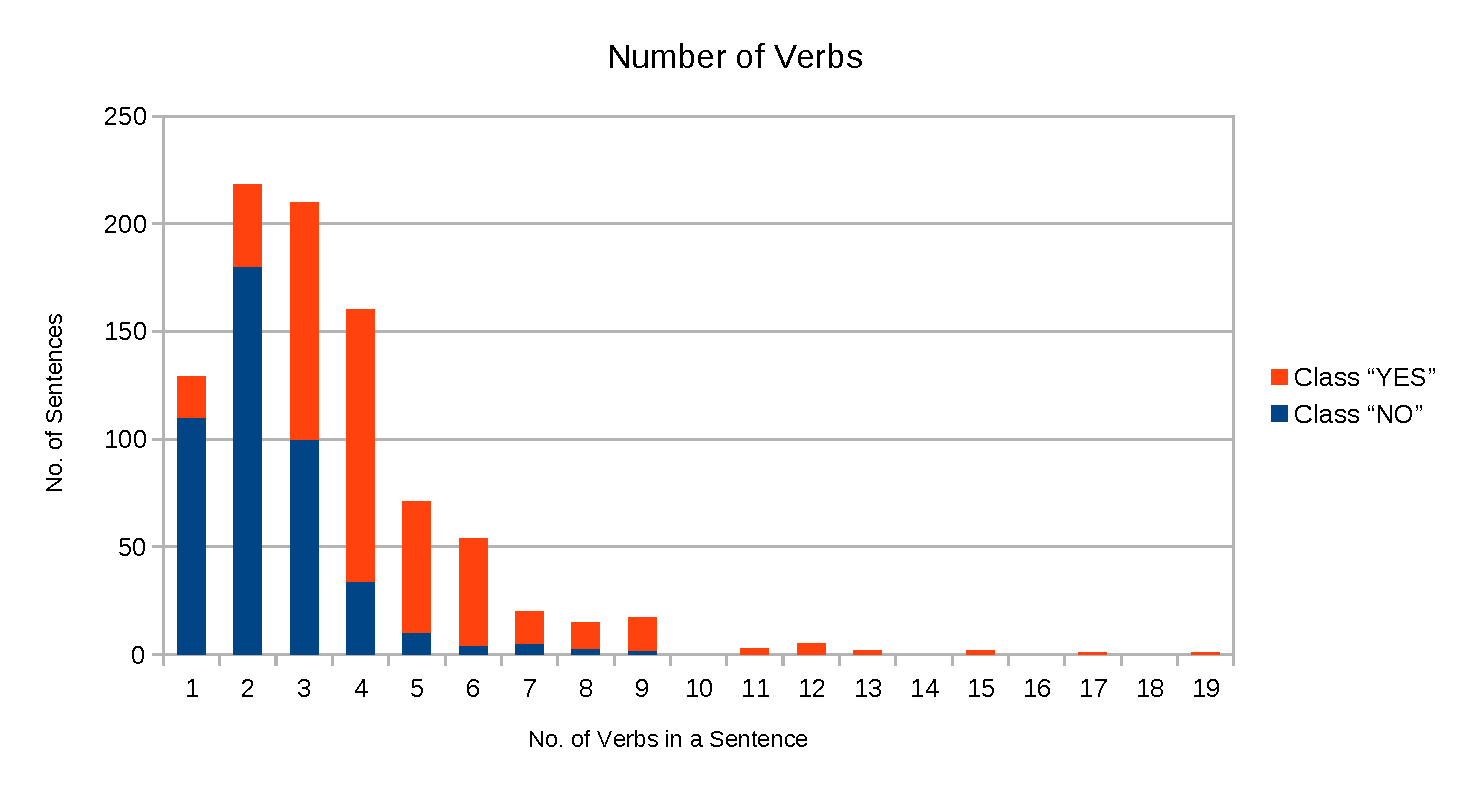
\includegraphics[width=0.8\linewidth]{figure/arguments/A_verbs1.pdf}
\caption{Argument Marker - Number of Verbs in a Sentence.}
\end{figure}

\begin{figure}[H]
\centering
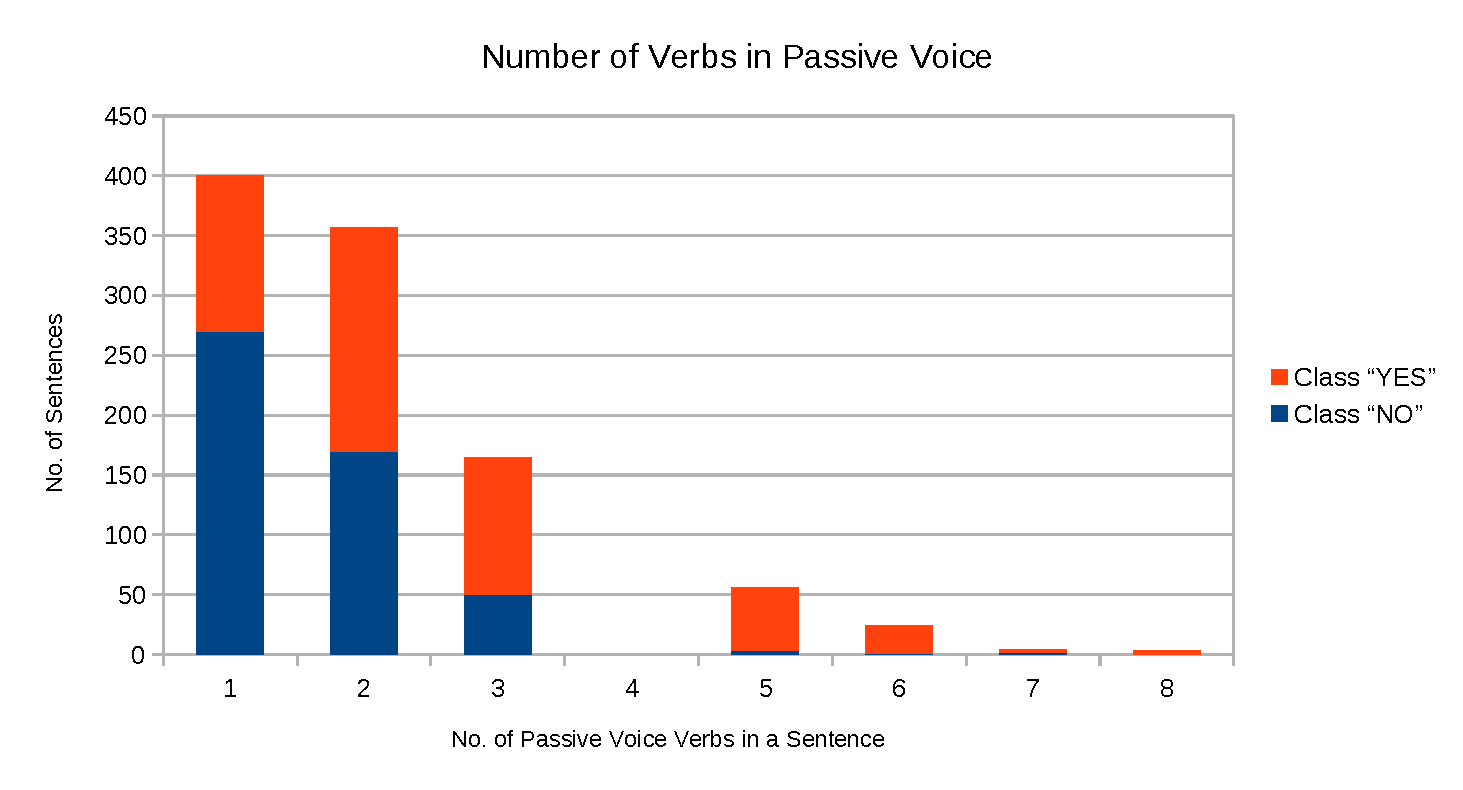
\includegraphics[width=0.8\linewidth]{figure/arguments/A_pv_verbs1.pdf}
\caption{Argument Marker - Number of Verbs in Passive Voice in a Sentence.}
\end{figure}

\begin{figure}[H]
\centering
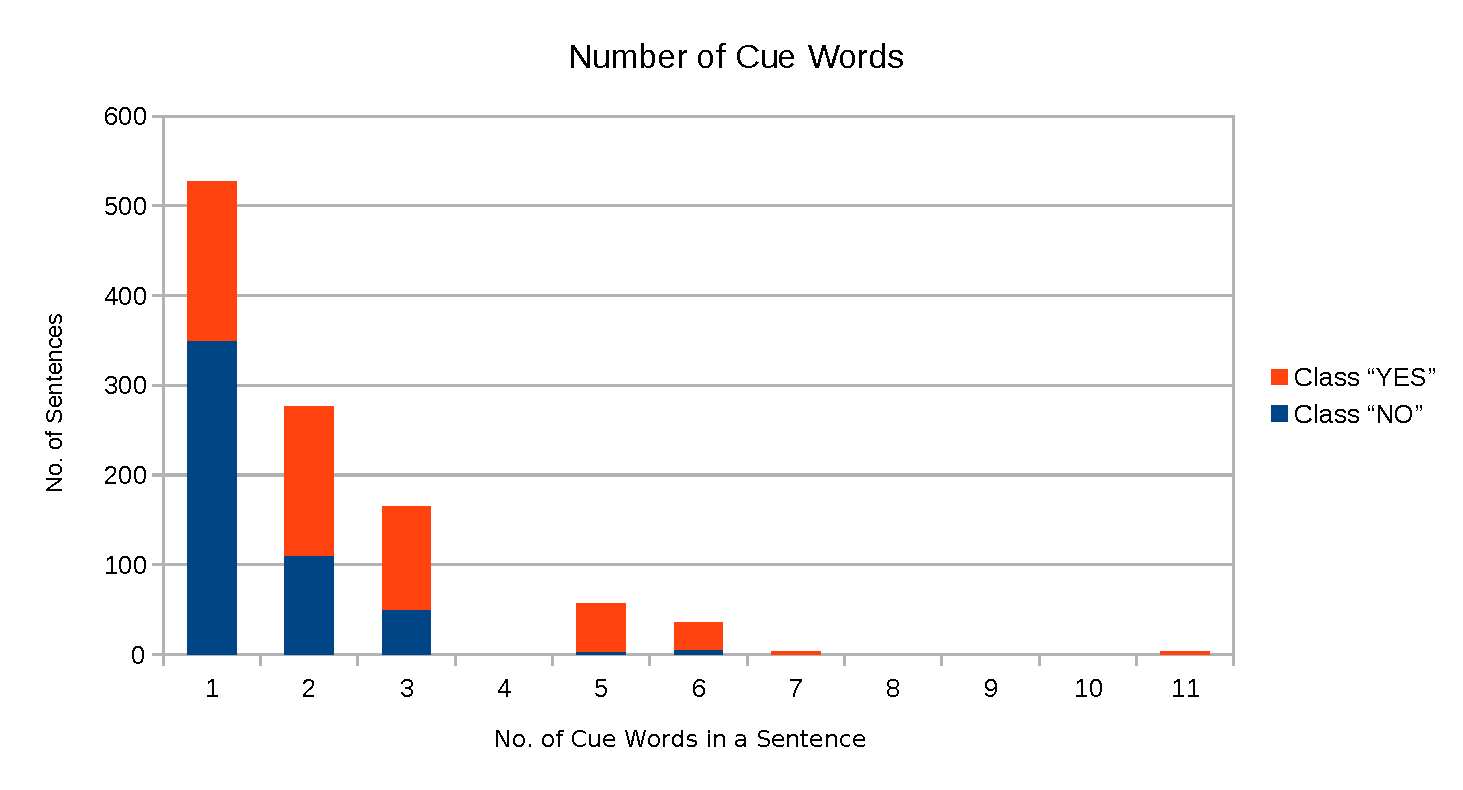
\includegraphics[width=0.8\linewidth]{figure/arguments/A_cue_words1.pdf}
\caption{Argument Marker - Number of Cue Words in a Sentence.}
\end{figure}

\begin{figure}[H]
\centering
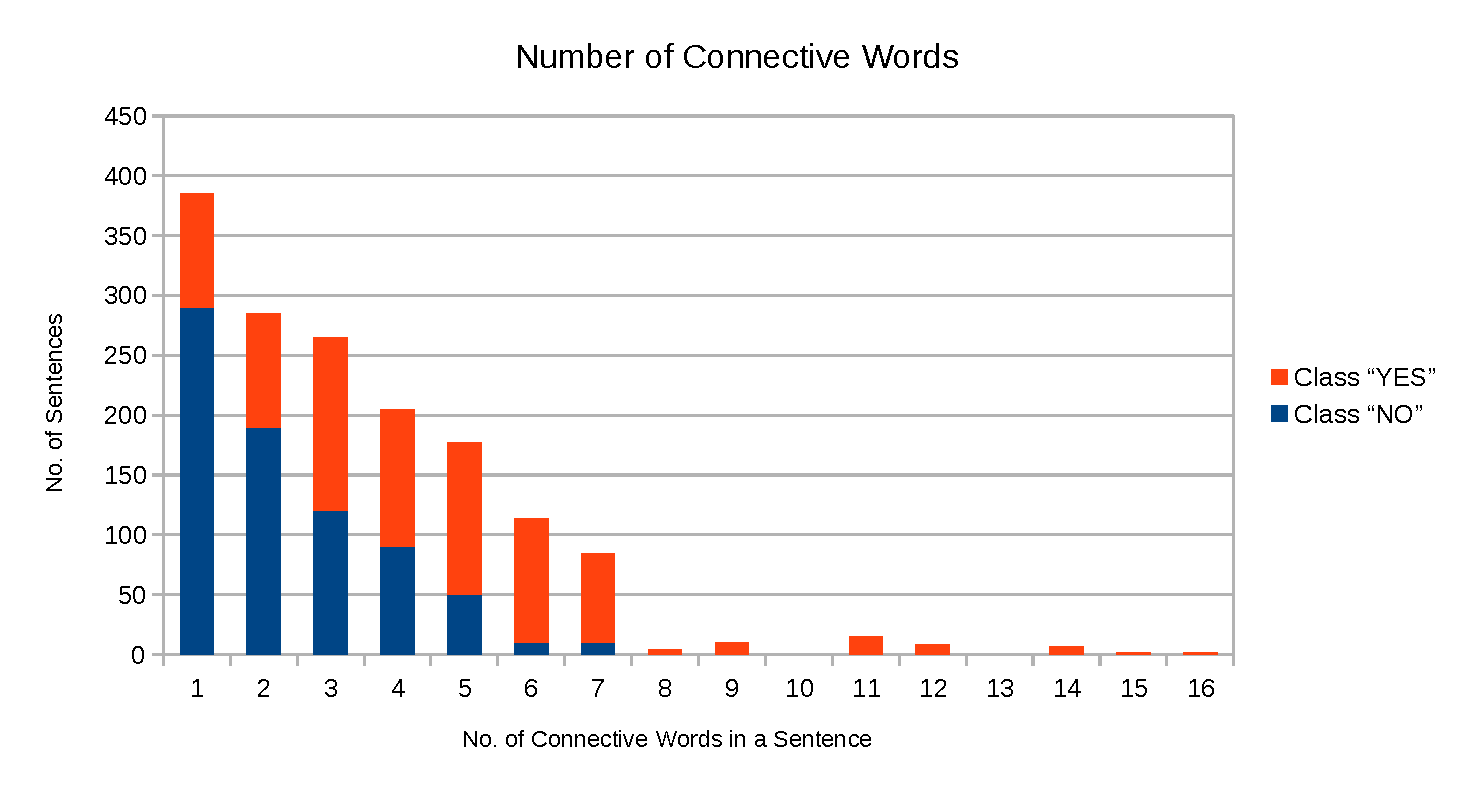
\includegraphics[width=0.8\linewidth]{figure/arguments/A_connective1.pdf}
\caption{Argument Marker - Number of Connective Words in a Sentence.}
\end{figure}

\begin{figure}[H]
\centering
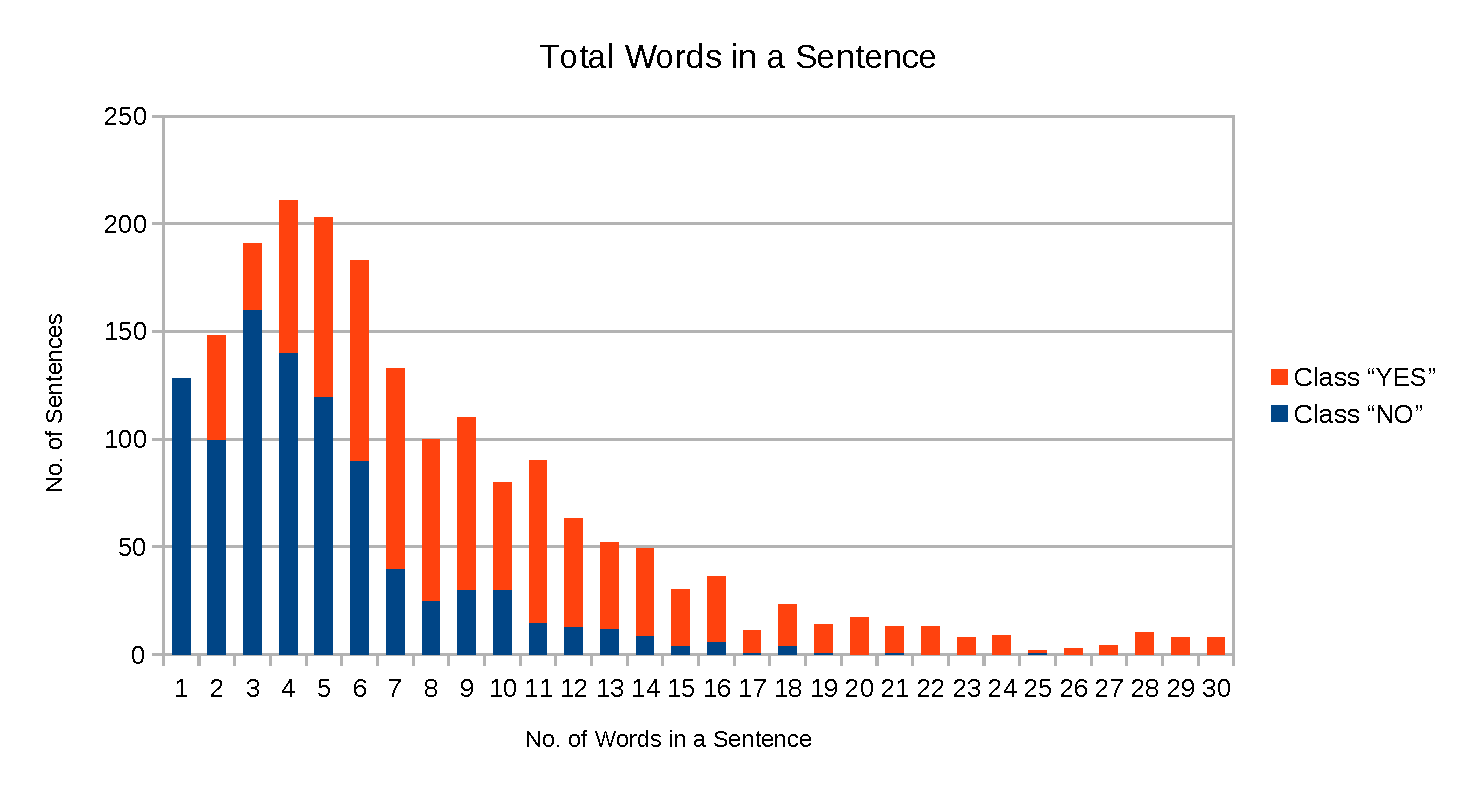
\includegraphics[width=0.8\linewidth]{figure/arguments/A_total_words1.pdf}
\caption{Argument Marker - Total words in a Sentence.}
\end{figure}

\begin{figure}[H]
\centering
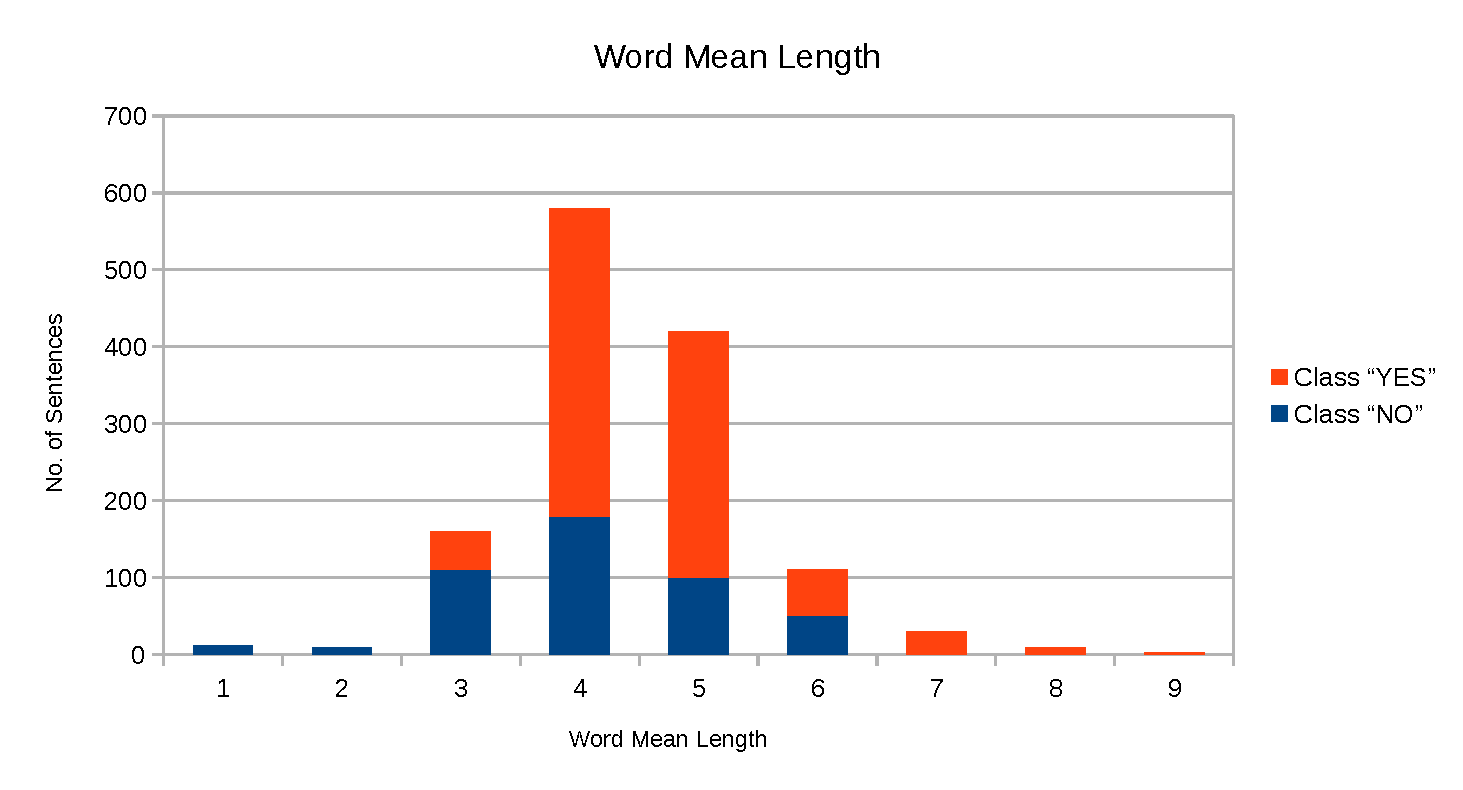
\includegraphics[width=0.8\linewidth]{figure/arguments/A_word_mean_length1.pdf}
\caption{Argument Marker - Word Mean Length.}
\end{figure}

\begin{figure}[H]
\centering
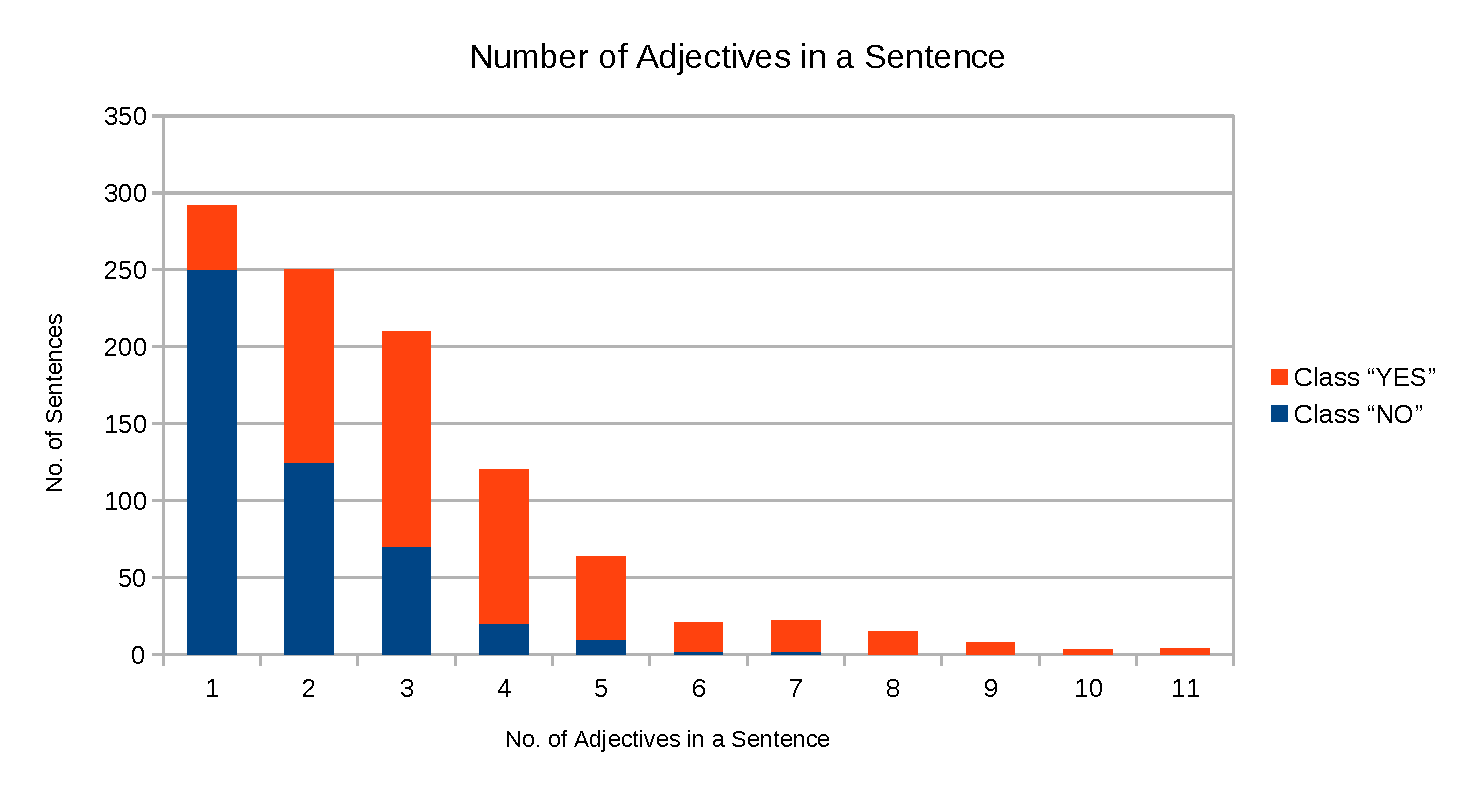
\includegraphics[width=0.8\linewidth]{figure/arguments/A_adjectives1.pdf}
\caption{Argument Marker - Number of Adjectives in a Sentence.}
\end{figure}

\begin{figure}[H]
\centering
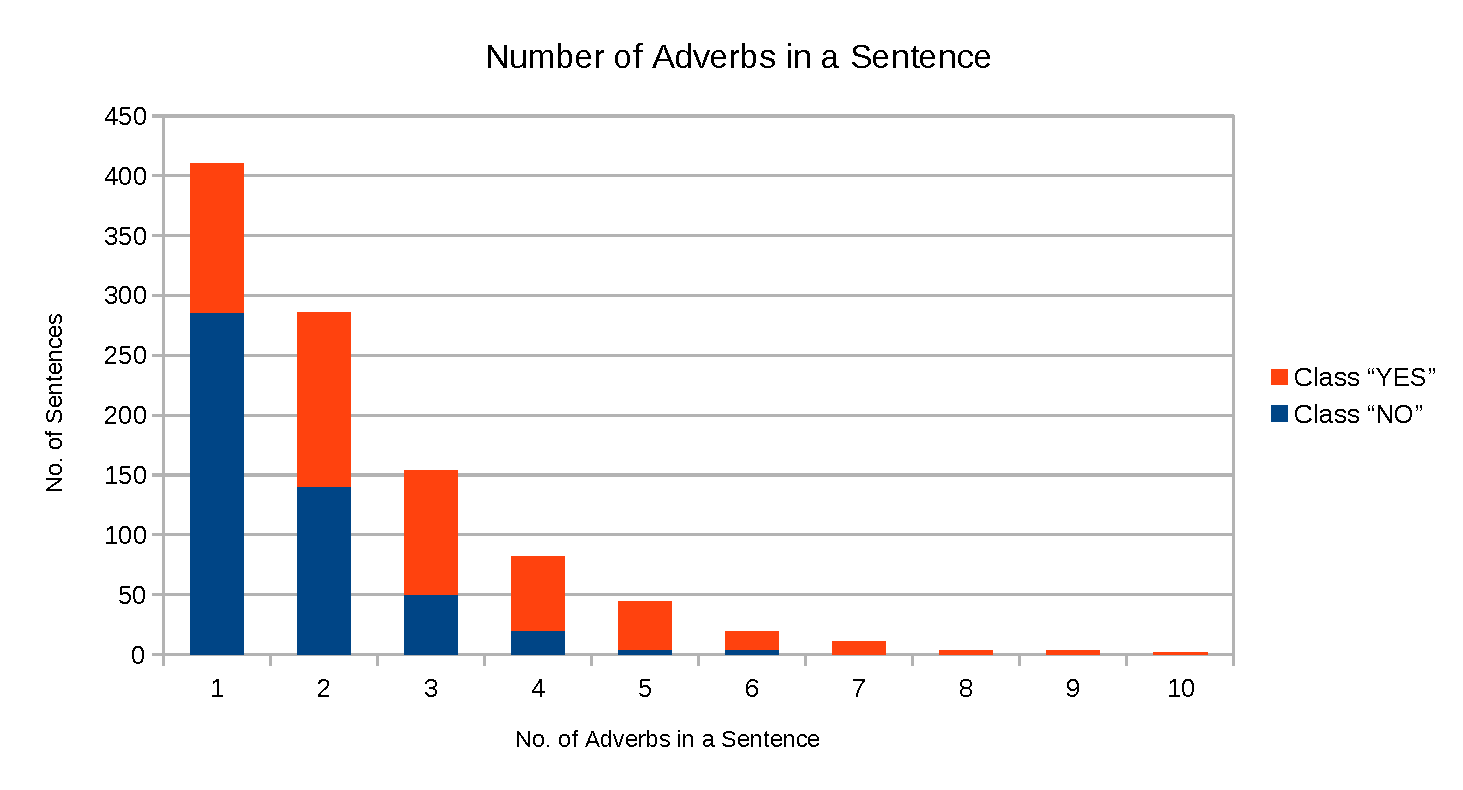
\includegraphics[width=0.8\linewidth]{figure/arguments/A_adverbs1.pdf}
\caption{Argument Marker - Number of Adverbs in a Sentence.}
\end{figure}

\begin{figure}[H]
\centering
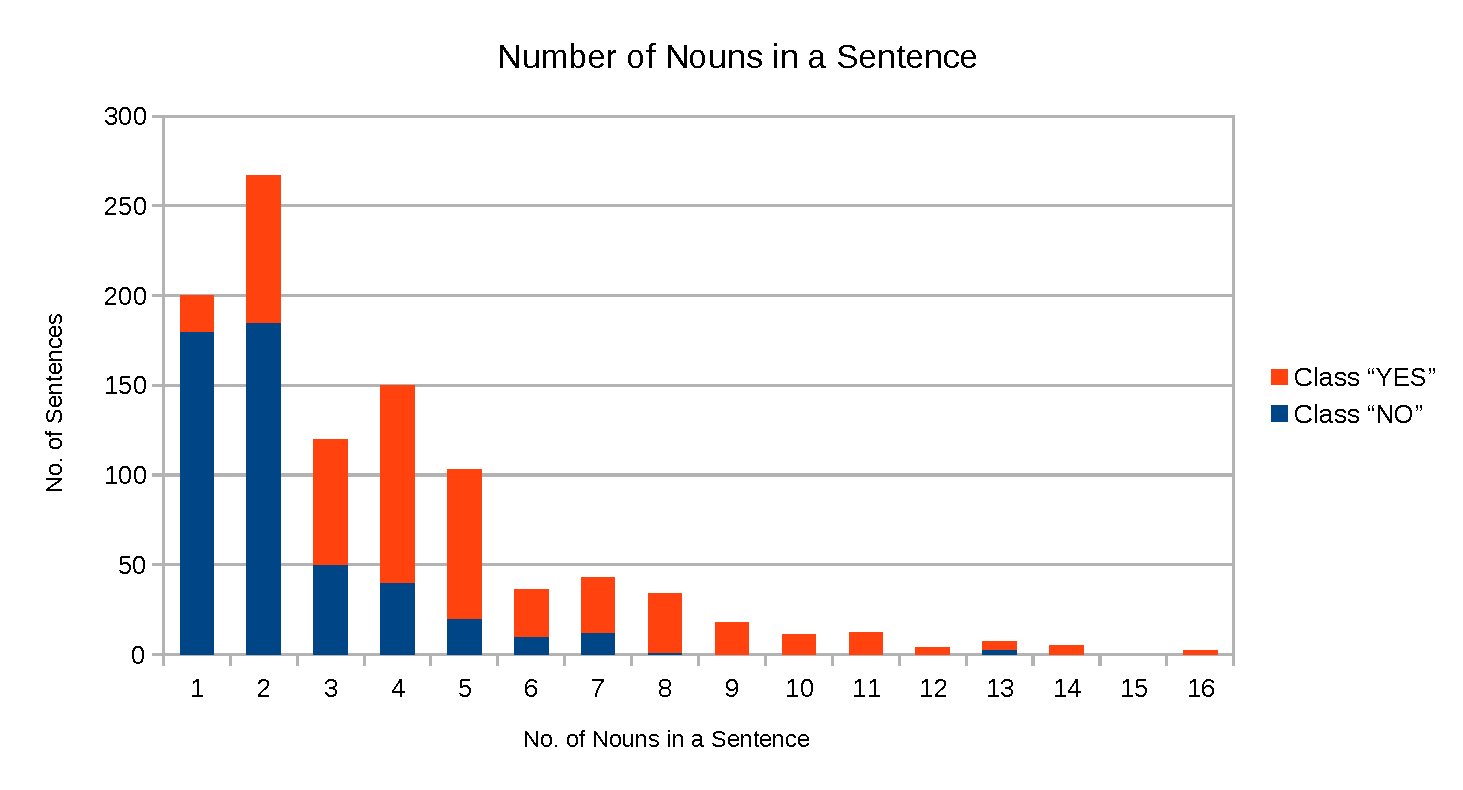
\includegraphics[width=0.8\linewidth]{figure/arguments/A_nouns1.pdf}
\caption{Argument Marker - Number of Nouns in a Sentence.}
\end{figure}

In all the above diagrams there is a common characteristic. As the frequency noted on X axis rises, we note that  ``Yes'' class transcendent ``No'' class (i.e. there are more sentences in ``Yes'' class.\\
\\
For example, in the (4.2) diagram, which shows the number of the verbs that exist in the sentences, we note that, as the number of the verbs rises, the red colour transcendents in each bar of the diagram.\\
\
But, especially for the example with the number of the verbs, there is one more interpretation, one of semantic nature. More precisely, we know that the verbs in a group of  two or three sentences have a defining role in the interpretation of the meaning, as they express an action. So, the more verbs there are in a group of sentences, the more possible it is a sentence contains arguments (to be characterised as Argumentative).\\
\\
But we have to note that not all the argument markers contribute in the same way in characterising a sentence as Argumentative. This is shown in the above diagrams and more precisely in those which have enough bars in which the red colour has the same size as the blue colour (there is an almost equal number of sentences between the two classes). A characteristic example is the ``No. of Connecting Words in a Sentence'' diagram (4.5). The markers which show this quality are used more for the fine tuning of the process.

\subsection{Algorithms used in Machine Learning Procedure}\label{412_ref}
In this subsection, we will see the results that the Algorithms which were used to check the accuracy of Machine Learning Process, produced. The results have been produced by carrying out classification on the Train Set and using ``10 Fold Cross Validation''\footnote{\url{https://en.wikipedia.org/wiki/Cross-validation_(statistics)}}.

\begin{table}[H]
\centering
\caption{Detailed Accuracy for Class “No” (Argument Extraction).}
\label{41_table_ref}
\begin{tabular}{cccc}
\hline
{\bf Algorithm}     & {\bf Precision} & {\bf Recall}    & {\bf F-Measure} \\ \hline
SVM                 & {\it 0.815}     & {\it 0.830}     & {\bf 0.823} \\
Random Forest       & {\bf 0.818} 	 & {\it 0.818}     & {\it 0.818}     \\
Native Bayes        & {\it 0.718}     & {\bf 0.899}     & {\it 0.798}     \\
Logistic Regression & {\it 0.801}     & {\it 0.819}     & {\it 0.819}     \\ \hline
\end{tabular}
\end{table}

\begin{table}[H]
\centering
\caption{Detailed Accuracy for Class “Yes” (Argument Extraction).}
\label{42_table_ref}
\begin{tabular}{cccc}
\hline
{\bf Algorithm}     & {\bf Precision} & {\bf Recall}    & {\bf F-Measure} \\ \hline
SVM                 & {\it 0.836}     & {\it 0.821}     & {\bf 0.828} \\
Random Forest       & {\it 0.827}     & {\bf 0.827}	   & {\it 0.827}     \\
Native Bayes        & {\bf 0.873} 	 & {\it 0.663}     & {\it 0.754}     \\
Logistic Regression & {\it 0.837}     & {\it 0.802}     & {\it 0.819}     \\ \hline
\end{tabular}
\end{table}

\begin{table}[H]
\centering
\caption{Weighted Average on both Classes (Argument Extraction).}
\label{43_table_ref}
\begin{tabular}{cccc}
\hline
{\bf Algorithm}     & {\bf Precision} & {\bf Recall}    & {\bf F-Measure} \\ \hline
SVM                 & {\bf 0.826} 	 & {\bf 0.826}     & {\bf 0.826} \\
Random Forest       & {\it 0.823}     & {\it 0.823}     & {\it 0.823}     \\
Native Bayes        & {\it 0.797}     & {\it 0.778}     & {\it 0.776}     \\
Logistic Regression & {\it 0.820}     & {\it 0.819}     & {\it 0.819}     \\ \hline
\end{tabular}
\end{table}

From the above tables, it is obvious that the best results were achieved by using the ``Support Vector Machines'' Algorithm. For this reason, we will look at some useful information  about this result straight away.

\begin{table}[H]
\centering
\caption{Additional Statistical Information (Argument Extraction).}
\label{44_table_ref}
\begin{tabular}{lll}
\hline
                                   & {\bf Frequenncy} & {\bf Percentage} \\ \hline
Correctly Classified Instances     & {\it 838}        & {\it 82.56\%}    \\
Incorrectly Classified Instances   & {\it 177}        & {\it 17.4383}    \\
Kappa statistic                    & {\it 0.6512}     & {\it -}          \\
Mean absolute error                & {\it 0.1744}     & {\it -}          \\
Root mean squared error            & {\it 0.4176}     & {\it -}          \\
Relative absolute error            & {\it -}          & {\it 34.90\%}    \\
Root relative squared error        & {\it -}          & {\it 83.54\%}    \\
Coverage of cases (0.95 level)     & {\it -}          & {\it 82.56\%}    \\
Mean rel. region size (0.95 level) & {\it -}          & {\it 50\%}       \\
Total Number of Instances          & {\it 1015}       & {\it -}          \\ \hline
\end{tabular}
\end{table}

We can also note that the results which all the algorithms that we tried produced  have small variations, they all produce approximately 0.8 F-Measure for both classes. A more important observation, though, is that the F-Measure for both classes (``Yes'', ``No'') also does not have many variations. This is especially important because in the dataset we studied, we noted that there is an equal partition between the sentences that are arguments and those which are not. Also, it is important because as it results from the above tables, the algorithms have the same ability to define correctly whether a sentence belongs to class ``Yes'' or class ``No''.

\subsection{Information about the Train Set}\label{413_ref}
One more measurement that was performed concerns the Train Set. More precisely, in the following diagram, the ``Error Rate'' in the ability to correctly characterize the sentences that are being analysed, appears. We can note that by using from 30\% of the Train Set (approximately 300 sentences) up to 100\%, the ``Error Rate'' is limited between 17.5\% - 18.3\%. For the next diagram, ``Support Vector Machines'' Algorithm was used.

\begin{figure}[H]
\centering
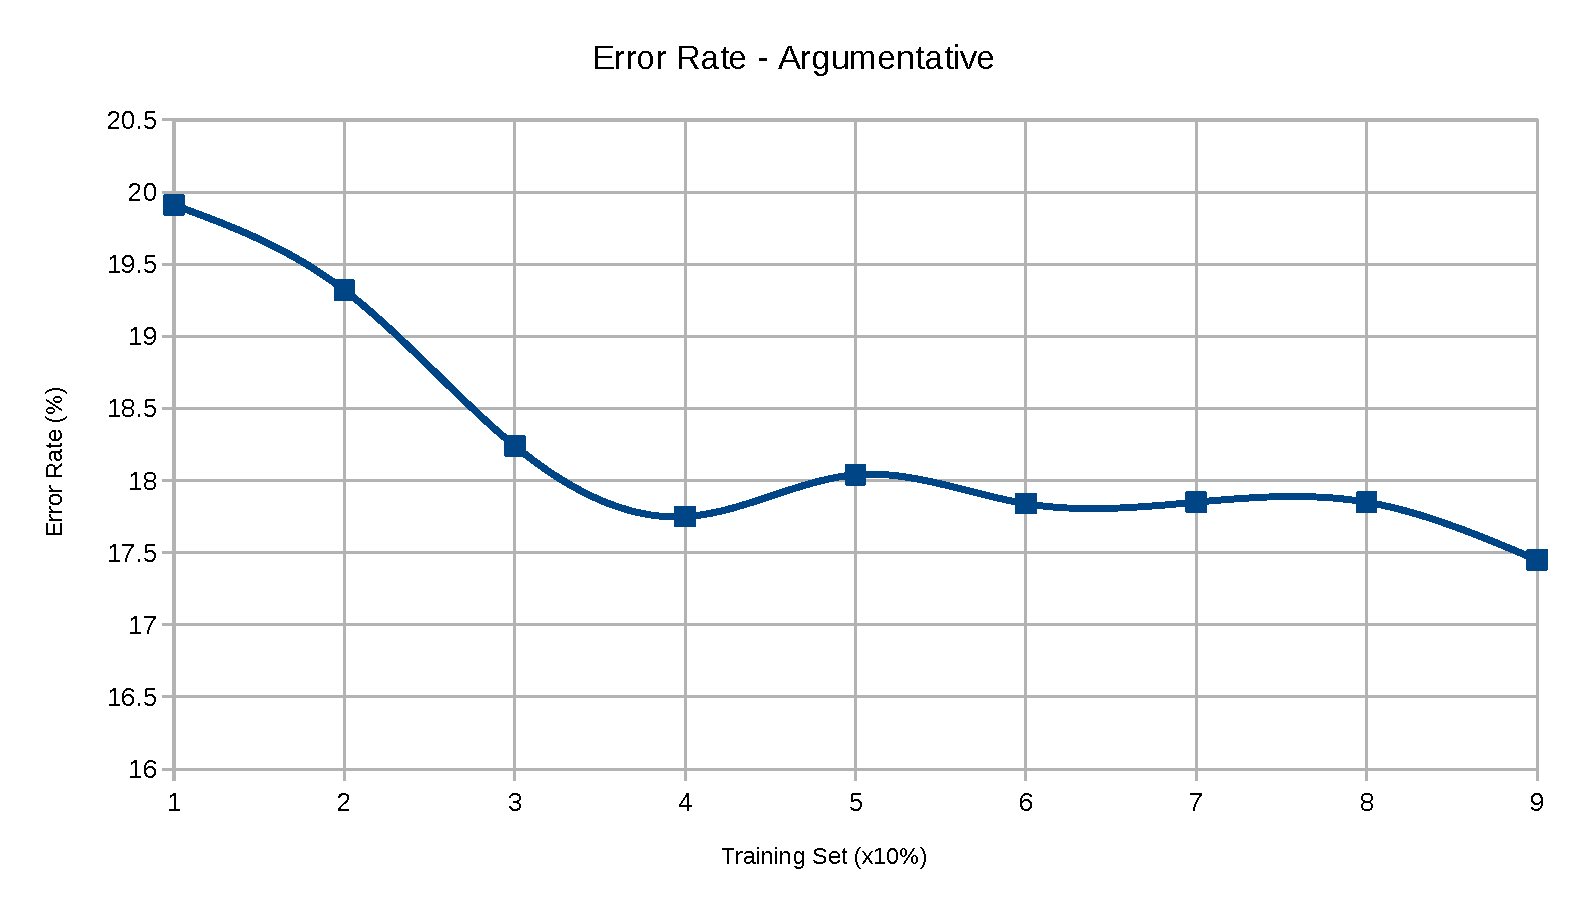
\includegraphics[width=1\linewidth]{figure/arguments/errorRate-argumentative}
\caption{Error Rate of Argumentative Sentence Classification.}
\end{figure}

\section{Suggestion Extraction}\label{42_ref}
For the confirmation of the results for extraction of the suggestions that the writers of the texts made, we needed to create two scenarios. Initially, we carried out ``10 Fold Cross Validation'' (\ref{421_ref}) on the Train Set. Next, we created a second scenario, according to which we divided the Train Set so that it contains an equal number of sentences that constitute suggestions and of sentences that do not. Next, we used this set as a Train Set and performed again the Machine Learning Process (\ref{422_ref}).

\subsection{``10 Fold Cross Validation'' on Train Set}\label{421_ref}
As described above, initially, we tried to apply ``10 Fold cross validation'' on the  Train Set. The results are shown in the following matrix:

\begin{table}[H]
\centering
\caption{Detailed Accuracy for Class “No” (Suggestion Extraction).}
\label{45_table_ref}
\begin{tabular}{cccc}
\hline
{\bf Algorithm} & {\bf Precision} & {\bf Recall} & {\bf F-Measure} \\ \hline
J48             & {\it 0.881}     & {\it 0.923}  & {\it 0.901}     \\
Random Forest   & {\it 0.890}      & {\it 0.915}  & {\it 0.902}     \\
Native Bayes    & {\bf 0.912}     & {\it 0.915}  & {\it 0.604}     \\
SVM             & {\it 0.839}     & {\bf 0.989}  & {\bf 0.908}     \\ \hline
\end{tabular}
\end{table}

\begin{table}[H]
\centering
\caption{Detailed Accuracy for Class “Yes” (Suggestion Extraction).}
\label{46_table_ref}
\begin{tabular}{cccc}
\hline
{\bf Algorithm} & {\bf Precision} & {\bf Recall} & {\bf F-Measure} \\ \hline
J48             & {\it 0.552}     & {\it 0.432}  & {\it 0.485}     \\
Random Forest   & {\it 0.556}     & {\it 0.489}  & {\it 0.519}     \\
Native Bayes    & {\it 0.608}     & {\bf 0.601}  & {\bf 0.604}     \\
SVM             & {\bf 0.735}     & {\it 0.137}  & {\it 0.230}     \\ \hline
\end{tabular}
\end{table}

\begin{table}[H]
\centering
\caption{Weighted Average on both Classes (Suggestion Extraction).}
\label{47_table_ref}
\begin{tabular}{cccc}
\hline
{\bf Algorithm} & {\bf Precision} & {\bf Recall} & {\bf F-Measure} \\ \hline
J48             & {\it 0.822}     & {\it 0.834}  & {\it 0.826}     \\
Random Forest   & {\it 0.830}      & {\it 0.837}  & {\it 0.833}     \\
Native Bayes    & {\bf 0.858}     & {\bf 0.858}  & {\bf 0.858}     \\
SVM             & {\it 0.820}      & {\it 0.835}  & {\it 0.786}     \\ \hline
\end{tabular}
\end{table}

From the above tables, we can see that the best results were achieved by using the ``Native Bayes'' Algorithm. For this reason, we will now see some useful information about this result.

\begin{table}[H]
\centering
\caption{Additional Statistical Information (Suggestion Extraction).}
\label{48_table_rer}
\begin{tabular}{lll}
\hline
                                   & {\bf Frequenncy} & {\bf Percentage} \\ \hline
Correctly Classified Instances     & {\it 871}        & {\it 85.81\%}    \\
Incorrectly Classified Instances   & {\it 144}        & {\it 14.19\%}    \\
Kappa statistic                    & {\it 0.518}      & {\it -}          \\
Mean absolute error                & {\it 0.1901}     & {\it -}          \\
Root mean squared error            & {\it 0.3382}     & {\it -}          \\
Relative absolute error            & {\it -}          & {\it 64.21\%}    \\
Root relative squared error        & {\it -}          & {\it 87.98\%}    \\
Coverage of cases (0.95 level)     & {\it -}          & {\it 95.67\%}    \\
Mean rel. region size (0.95 level) & {\it -}          & {\it 70.64\%}    \\
Total Number of Instances          & {\it 1015}       & {\it -}          \\ \hline
\end{tabular}
\end{table}

The above results have been produced by executing ``10 Fold cross validation'' on the Trainset we created, whereas in the arguments section we noticed that a relatively small percentage of the sentences (almost 20\%) is enough to stabilise the error rate at a low level. In this case, however, the same thing doesn't happen. We see that the algorithms that were applied  have an extremely good ability to correctly characterise the sentences of the text that are not suggestions. In case, however, we want to characterise a sentence as a suggestion, there is a weakness, and low results (approximately 0.5 in the F-measure scale), are produced. This matter is especially important because it suggests that the algorithms in reality cannot characterise a sentence correctly as a suggestion or not.\\
\\
The main reason why this particularity occurs (good percentages for class ``No'', lower percentages for class ``Yes'' is that  the Trainset on which ``10 Fold cross validation'' was executed, created  very few sentences that are characterised as suggestions, so only a small sample was chosen during the execution of ``10 Fold cross validation''. To better understand this problem, we should think about the following.\\
\\
During the execution of ``10 fold cross validation'', the total of the data is divided in ten parts and then a part is chosen as a train set and the rest of the total as the test set. In our case, we had a sample of approximately 100 sentences as the train set, which contained very few sentences which are suggestions (in total there were about 170 sentences). So, in order to overcome the above problem and to be able to check if the process that was executed was correct, we tried a different tactic,which will be described in the next unit (\ref{422_ref}).

\subsection{Equivalent Train Set}\label{422_ref}
In the second scenario, a different Train Set was used. We divided the Train Set in a way that it contains equal amount of sentences that can be characterised as suggestions, compared to those that cannot. The reason is that the Train Set contains relatively less entries that refer to suggestions compare to the sentences that do not constitute suggestions. So, we used a corpus that contained two hundred sentences that are characterised as suggestions and two hundred more that are not. Next, we used this set as a Train Set and as a Test Set we used the whole corpus. The results are shown in the following tables:
\begin{table}[H]
\centering
\caption{Detailed Accuracy for Class “No” (Suggestion Extraction, using Equivalent Train Set).}
\label{49_table_rer}
\begin{tabular}{cccc}
\hline
{\bf Algorithm} & {\bf Precision} & {\bf Recall} & {\bf F-Measure} \\ \hline
J48             & {\it 0.940}      & {\it 0.810}   & {\it 0.870}      \\
Random Forest   & {\bf 0.996}     & {\it 0.810}   & {\bf 0.893}     \\
Native Bayes    & {\it 0.941}     & {\bf 0.828}  & {\it 0.881}     \\
SVM             & {\it 0.939}     & {\it 0.819}  & {\it 0.875}     \\ \hline
\end{tabular}
\end{table}

\begin{table}[H]
\centering
\caption{Detailed Accuracy for Class “Yes” (Suggestion Extraction, using Equivalent Train Set).}
\label{410_table_rer}
\begin{tabular}{cccc}
\hline
{\bf Algorithm} & {\bf Precision} & {\bf Recall} & {\bf F-Measure} \\ \hline
J48             & {\it 0.470}      & {\it 0.765}  & {\it 0.582}     \\
Random Forest   & {\bf 0.533}     & {\bf 0.984}  & {\bf 0.641}     \\
Native Bayes    & {\it 0.495}     & {\it 0.765}  & {\it 0.601}     \\
SVM             & {\it 0.479}     & {\it 0.760}   & {\it 0.588}     \\ \hline
\end{tabular}
\end{table}

\begin{table}[H]
\centering
\caption{Weighted Average on both Classes (Suggestion Extraction, using Equivalent Train Set).}
\label{411_table_rer}
\begin{tabular}{cccc}
\hline
{\bf Algorithm} & {\bf Precision} & {\bf Recall} & {\bf F-Measure} \\ \hline
J48             & {\it 0.855}     & {\it 0.802}  & {\it 0.818}     \\
Random Forest   & {\bf 0.912}     & {\bf 0.841}  & {\bf 0.857}     \\
Native Bayes    & {\it 0.861}     & {\it 0.817}  & {\it 0.831}     \\
SVM             & {\it 0.856}     & {\it 0.808}  & {\it 0.823}     \\ \hline
\end{tabular}
\end{table}

From the above tables we can see that the best results were achieved by using the ``Random Forest'' Algorithm.

\begin{table}[H]
\centering
\caption{Additional Statistical Information (Suggestion Extraction, using Equivalent Train Set).}
\label{412_table_rer}
\begin{tabular}{ccc}
\hline
                                   & {\bf Frequenncy} & {\bf Percentage} \\ \hline
Correctly Classified Instances     & {\it 854}        & {\it 84.14\%}    \\
Incorrectly Classified Instances   & {\it 161}        & {\it 15.86\%}    \\
Kappa statistic                    & {\it 0.5966}     & {\it -}          \\
Mean absolute error                & {\it 0.2273}     & {\it -}          \\
Root mean squared error            & {\it 0.3467}     & {\it -}          \\
Relative absolute error            & {\it -}          & {\it 47.98\%}    \\
Root relative squared error        & {\it -}          & {\it 73.02\%}    \\
Coverage of cases (0.95 level)     & {\it -}          & {\it 97.14\%}    \\
Mean rel. region size (0.95 level) & {\it -}          & {\it 83.00\%}    \\
Total Number of Instances          & {\it 1015}       & {\it -}          \\ \hline
\end{tabular}
\end{table}

We observe that the method we chose in order to define our train set, succeeded much better results. Still, even if the results are quite satisfying, we are of the opinion that an even better result is possible.

%\section{Overall Opinion Extraction}\label{43_ref}
%For the third part of this Thesis, an extensive evaluation did not take place because the dataset we processed did not contain sufficient data. More precisely, almost all users' texts express a negative opinion, subsequently there is only a small number of texts that can be characterised as presenting a positive opinion. This fact creates doubts about the quality of the process. To be more precise, the measurements we carried out show that the results are realistic enough, i.e. the majority of the sentences were characterised as ``Negative''. On the other hand, we cannot make an evaluation about the sentences that are characterised as ``Positive''

